\section{Modelling}
	Efficiency of a GC is defined as the ratio of useful write vs. actual write. Useful write is defined as the amount of data passed to the write API of the file system and Actual write is the sum of amount of data moved, blocks erased and the useful write. A good GC is one which is able to find space to write data quickly. It has to do so by spreading the writes evenly across the various blocks in the flash (wear-leveling). Writing too often to a particular block can cause the flash to wear-out quickly. 

	Another important criterion in choosing a certain GC is the traffic pattern of the data. Data can be written to the flash in short bursts or can be spread out evenly. They tend to follow statistical patterns such as Uniform, Normal or Bi-Modal. For the current project, there are no sets of real-world applications which can be used to test the GC algorithms. So, one of the goals of the project is to create a set of pseudo applications which generates data that follows a Uniform, Normal or a Bi-Modal type of distribution.

Five different GC algorithms are considered which has been described below. The first two are round-robin style of GCs while the other three are generational type of algorithms.
\begin{itemize}
\item FIFE – First Insert First Erase:
The data is always written starting from the first block and when the flash reaches a pre-defined fullness level, the GC is invoked. The GC compacts the oldest block and keeps moving forward along the blocks until sufficient space is created to store the record. The GC returns an error when even after traversing the blocks, it is not able to find sufficient space. 
\item LAC – Least Active Clean:
When the GC is invoked, it finds out the block that has the least amount of active records and compacts that block. The compacted block is then used for the next write operation.
\item 3-Generation:
In this GC, the entire flash is divided into three generations. The ratio of the blocks in each generation can be 12:3:1 or 4:3:1. Data is always written to the first generation and when it becomes full, the active records are moved to the 2nd generation. When the 2nd generation becomes full, its active records are moved to the 3rd generation. This allows the GC to separate the hot from the cold data. The intuition is that this reduces the amount of movement of the active records which is a draw-back of the round-robin algorithms.
\item N-Generation:
All the blocks in the flash is considered as a generation in this algorithm. Cold data is always pushed to the highest possible generation.
\item Eta-N-Generation:
This is similar to the N-Gen algorithm, except that the amount of data that is moved is decided by a factor called Eta. Eta denotes the fullness level of the flash when the GC is invoked.
\item Gamma-N-Generation:
\end{itemize}	


The GC that will be implemented will be the one that has the best efficiency for all three traffic patterns. Depending on the outcome of this project, a single GC might be implemented or a hybrid approach will be chosen where one type of GC is used for certain fullness levels and another type for other levels of fullness.

\begin{figure}
\centering
\subfloat[]{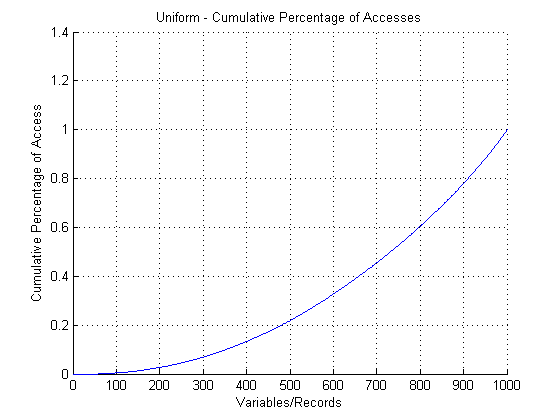
\includegraphics[width=3.1in]{C:/Ananth/OSU/CETI/MS-Thesis/MS-thesis-Report/imgs/Uniform-CumulAccess.png}} 
\subfloat[]{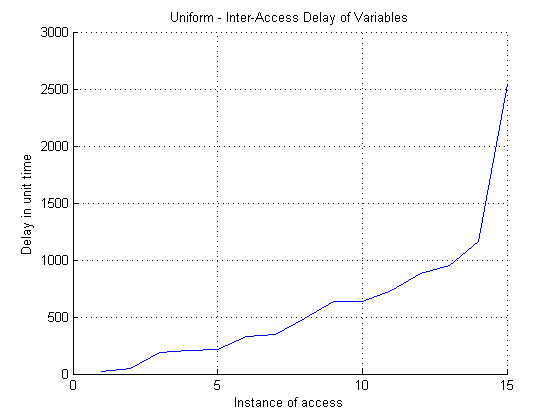
\includegraphics[width=3.1in]{C:/Ananth/OSU/CETI/MS-Thesis/MS-thesis-Report/imgs/Uniform-InterAccessDelay.png}}
\caption{Potential for 0.5 V bias.} 
\label{fig:EcUND} 
\end{figure} 

\comment{
\begin{figure}[ht]
\begin{minipage}[b]{0.4\linewidth}
\centering
	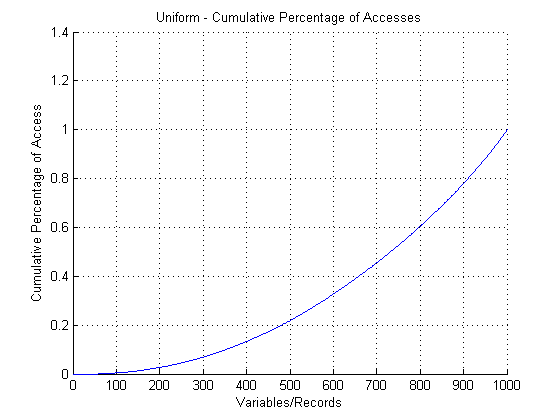
\includegraphics [width=\textwidth] {C:/Ananth/OSU/CETI/MS-Thesis/MS-thesis-Report/imgs/Uniform-CumulAccess.png}
	\captionof{figure}{Cumulative accesses for all variables that follow Uniform distribution}
	\label{UniformCumul}
\end{minipage}
\hspace{0.5cm}

\begin{minipage}[b]{0.4\linewidth}
\centering
	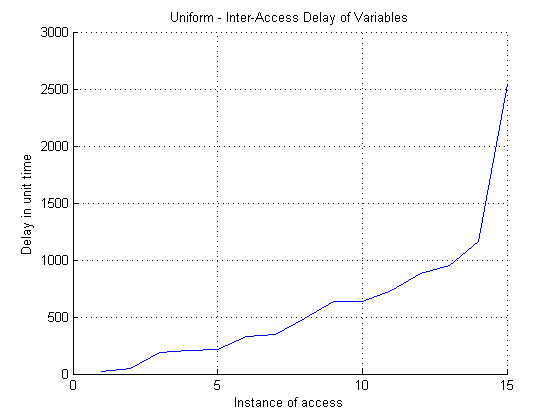
\includegraphics [width=\textwidth] {C:/Ananth/OSU/CETI/MS-Thesis/MS-thesis-Report/imgs/Uniform-InterAccessDelay.png}
	\captionof{figure}{Inter-access delay for all variables that follow Uniform distribution}
	\label{UniformCumul}
\end{minipage}
\end{figure}
}

\noindent
\begin{minipage}{\linewidth}
\makebox[\linewidth]{
    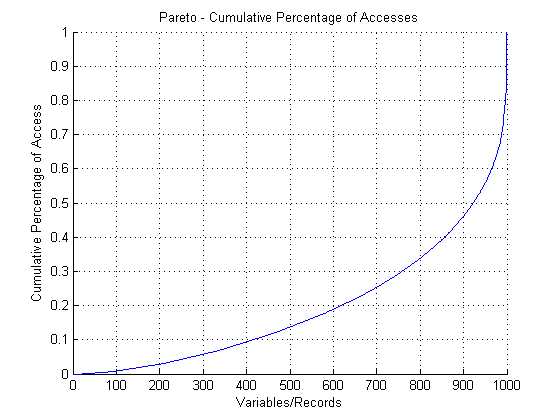
\includegraphics [keepaspectratio=true, scale = 0.6] {C:/Ananth/OSU/CETI/MS-Thesis/MS-thesis-Report/imgs/Pareto-CumulAccess.png}}
\captionof{figure}{Cumulative accesses for all variables that follow Pareto distribution}
\label{UniformCumul}
\end{minipage}

\noindent
\begin{minipage}{\linewidth}
\makebox[\linewidth]{
    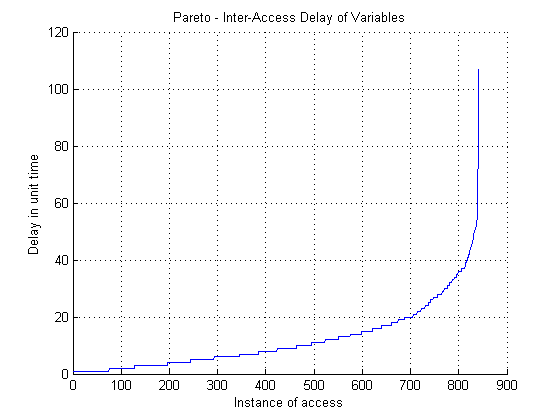
\includegraphics [keepaspectratio=true, scale = 0.6] {C:/Ananth/OSU/CETI/MS-Thesis/MS-thesis-Report/imgs/Pareto-InterAccessDelay.png}}
\captionof{figure}{Inter-access delay for all variables that follow Pareto distribution}
\label{UniformCumul}
\end{minipage}

